%%%%%%%%%%%%%%%%%%%%%%%%%%%%%%%%%%%%%%%%%%%%%%%%
% Python Cheat Sheet
% baposter Landscape Poster
% LaTeX Template
% Version 1.0 (11/06/13)
% baposter Class Created by:
% Brian Amberg (baposter@brian-amberg.de)
% This template has been downloaded from:
% http://www.LaTeXTemplates.com
% License:
% CC BY-NC-SA 3.0 (http://creativecommons.org/licenses/by-nc-sa/3.0/)
% Edited by Michelle Cristina de Sousa Baltazar
%%%%%%%%%%%%%%%%%%%%%%%%%%%%%%%%%%%%%%%%%%%%%%%%

%----------------------------------------------------------------
%   PACKAGES AND OTHER DOCUMENT CONFIGURATIONS
%----------------------------------------------------------------

\documentclass[landscape,a0paper,fontscale=0.285]{baposter} % Adjust the font scale/size here
\title{To be in season or not to be in season}
\usepackage[utf8]{inputenc}

\usepackage{graphicx} % Required for including images
\graphicspath{{figures/}} % Directory in which figures are stored

\usepackage{float}

\usepackage{xcolor}
\usepackage{colortbl}
\usepackage{tabu}

\usepackage{mathtools}
%\usepackage{amsmath} % For typesetting math
\usepackage{amssymb} % Adds new symbols to be used in math mode

\usepackage{booktabs} % Top and bottom rules for tables
\usepackage{enumitem} % Used to reduce itemize/enumerate spacing
\usepackage{palatino} % Use the Palatino font
\usepackage[font=small,labelfont=bf]{caption} % Required for specifying captions to tables and figures

\usepackage{multicol} % Required for multiple columns
\setlength{\columnsep}{1.5em} % Slightly increase the space between columns
\setlength{\columnseprule}{0mm} % No horizontal rule between columns

\usepackage{tikz} % Required for flow chart
\usetikzlibrary{decorations.pathmorphing}
\usetikzlibrary{shapes,arrows} % Tikz libraries required for the flow chart in the template

\newcommand{\compresslist}{ % Define a command to reduce spacing within itemize/enumerate environments, this is used right after \begin{itemize} or \begin{enumerate}
\setlength{\itemsep}{1pt}
\setlength{\parskip}{0pt}
\setlength{\parsep}{0pt}
}

\definecolor{lightblue}{rgb}{0.145,0.6666,1} % Defines the color used for content box headers

\begin{document}

\begin{poster}
{
headerborder=closed, % Adds a border around the header of content boxes
colspacing=0.8em, % Column spacing
bgColorOne=white, % Background color for the gradient on the left side of the poster
bgColorTwo=white, % Background color for the gradient on the right side of the poster
borderColor=lightblue, % Border color
headerColorOne=black, % Background color for the header in the content boxes (left side)
headerColorTwo=lightblue, % Background color for the header in the content boxes (right side)
headerFontColor=white, % Text color for the header text in the content boxes
boxColorOne=white, % Background color of the content boxes
textborder=roundedleft, % Format of the border around content boxes, can be: none, bars, coils, triangles, rectangle, rounded, roundedsmall, roundedright or faded
eyecatcher=true, % Set to false for ignoring the left logo in the title and move the title left
headerheight=0.15\textheight, % Height of the header
headershape=roundedright, % Specify the rounded corner in the content box headers, can be: rectangle, small-rounded, roundedright, roundedleft or rounded
headerfont=\Large\bf\textsc, % Large, bold and sans serif font in the headers of content boxes
%textfont={\setlength{\parindent}{1.5em}}, % Uncomment for paragraph indentation
linewidth=2pt % Width of the border lines around content boxes
}
%----------------------------------------------------------------
%   TÍTULO
%----------------------------------------------------------------
{\bf\textsc{To be in season or not to be in season}\vspace{0.5em}} % Poster title
{\textsc{ To be in season or not to be in season \hspace{20pt}}}
{\textsc{ Ekaterina Dopiro, Fabien Zellweger \& Christopher Benz \\ 
\includegraphics[scale=0.3]{img/EPFL-Logo-RVB-55.jpg} \hspace{6pt}}} 


%------------------------------------------------
% BÁSICO DO PYTHON
%------------------------------------------------
\headerbox{Data Scraping:}{name=objectives,column=0,row=0}{

%--------------------------------------
\colorbox[HTML]{CCFFFF}{\makebox[\textwidth-2\fboxsep][l]{\bf - Introduction:}}
Humankind has acquired knowledge about food for ages. As a result we know that each food has its season. However with the rise of civilization we are no longer dependent on it as any food can be transported to any point in the world.\\
The question is then: how much food do we consume out of the season? Our project focuses on two aspects: the season the foods are naturally produced, and the area where they are naturally produced.

\colorbox[HTML]{CCFFFF}{\makebox[\textwidth-2\fboxsep][l]{\bf - Data Scraping:}}
The first challenge of our project is to get a lot of recipes including their ingredient list and the review dates. We also need the seasons of those ingredients as well as their states of origin.

\begin{itemize}
\item Extract review date from our 3 most present websites (allrecipes.com, food.com and foodnetwork.com).
\item Extract the corresponding ingredient list on our dataset.
\item Extract month per ingredient from different source, including, if possible, the states (eattheseasons.com, seasonalfoodguide.org).
\end{itemize}

\begin{figure}[H]  
  \centering
    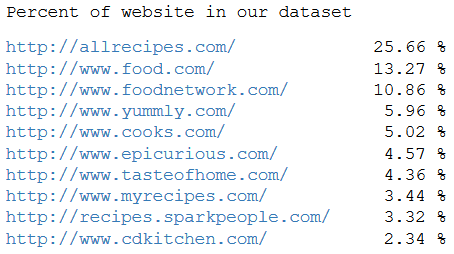
\includegraphics[scale=0.6]{img/percent.png}
    \caption{The proportion of the 10 biggest websites in our dataset. Given this distibution, we choose to only take care of the top 3.}
\end{figure}


\vspace{0.0em} % When there are two boxes, some whitespace may need to be added if the one on the right has more content
}

%------------------------------------------------
% Lógica Básica do Python
%------------------------------------------------

\headerbox{Data Processing}{name=introduction,column=1,row=0,bottomaligned=objectives}{

\colorbox[HTML]{CCFFFF}{\makebox[\textwidth-2\fboxsep][l]{\bf - Scoring:}}

We introduce a score in order to rank the food consumption as seasonal or not.
For a given food, a score is computed for each month of the year: the score is equal to 6 minus the number of months to the closest month when that food is consumed.\\
\begin{equation}
   S_i \in [0,6] , i \in [1,12]
\end{equation}
\begin{equation}
   S_i = 6 - [\#\text{months to closest seasonal month}]
\end{equation}
Estimates the distance in time and place to the optimal climate for the production of the given food.
\linebreak
Then, for the recipe score, we take the mean food score on all foods in the recipe.

\begin{figure}[H]
 \centering
    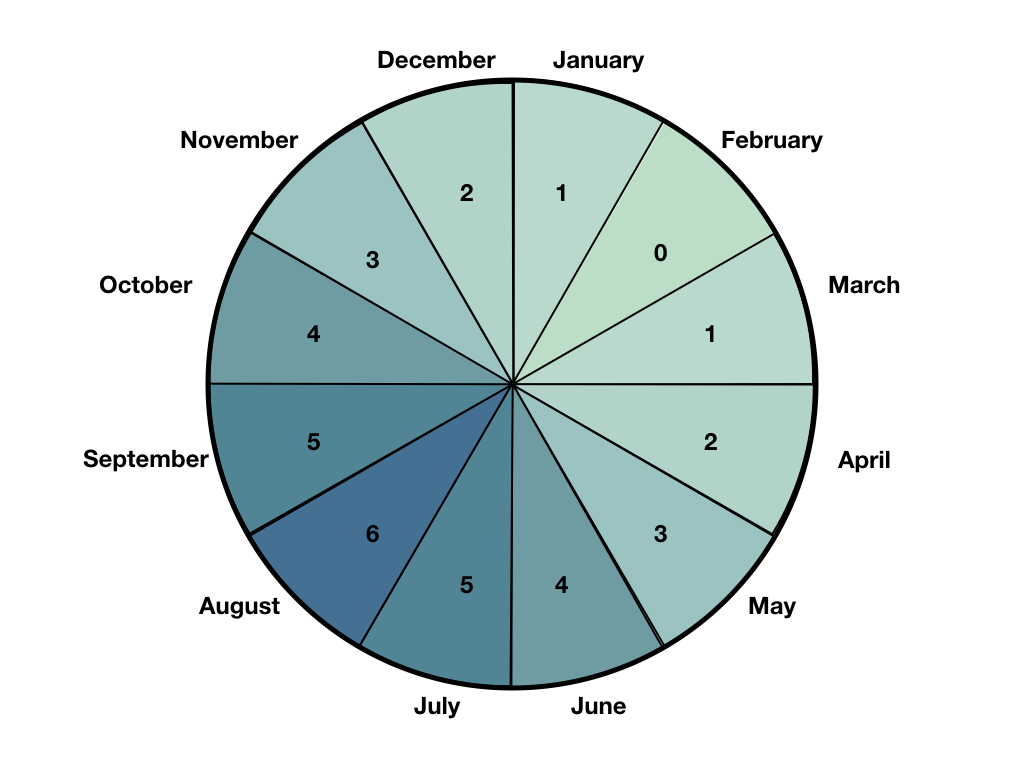
\includegraphics[scale=0.16]{img/Month_Disc001.jpeg}
    \caption{The score for a food which is seasonal on August}
\end{figure}

\colorbox[HTML]{CCFFFF}{\makebox[\textwidth-2\fboxsep][l]{\bf - Words matching:}}

The list of ingredients for a recipe contains a lot of noisy data, e.g. in 'one and a half tablespoons of black pepper', we are only interested in 'black pepper'. Therefore, for matching between the two datasets, we search for any occurence of the food name in the recipe ingredient list. This causes issues for double-worded foods (e.g. 'sweet potato') because it matches both on 'sweet potato' and 'potato'.
}


%------------------------------------------------
% Listas no Python
%------------------------------------------------

\headerbox{Results}{name=results,column=2,span=2,row=0}{

\colorbox[HTML]{CCFFFF}{\makebox[\textwidth-2\fboxsep][l]{\bf - Results:}}
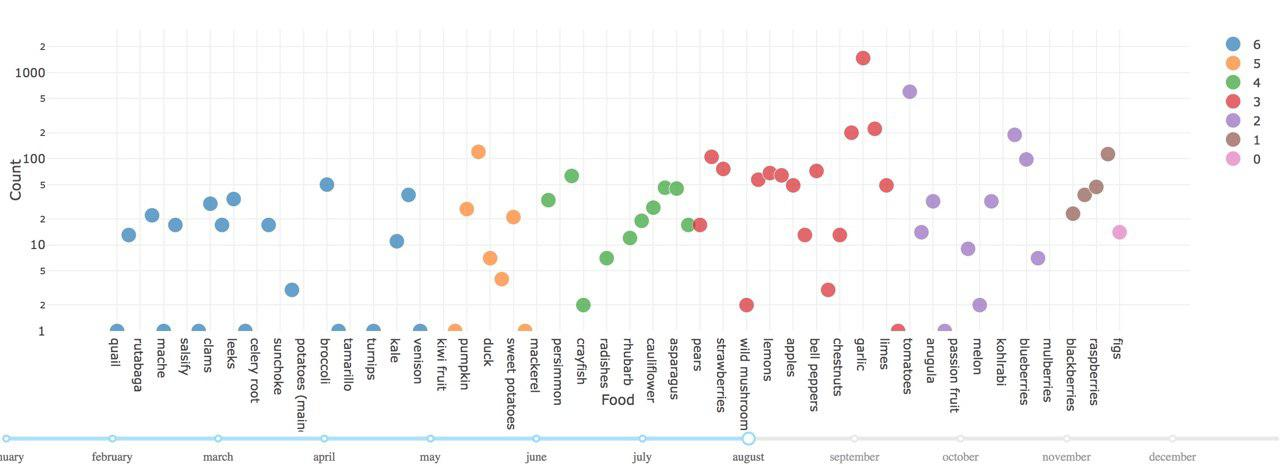
\includegraphics[scale=0.35]{img/photo_2018-01-22_10-51-41.jpg}
\linebreak \\
Our visualization results allow us to observe some facts about the data. For example:
- Garlic seems to be highly consumed no matter the season, compared to other foods. This could be explained by the fact that it is usually used as a spice, and that people love garlic bread all year long.
- Consumption at the correct season seems to dominate during the late winter and spring months, while during summer and autumn there is much more un-seasonal consumption.
\linebreak \\
**Bullshit citations
\linebreak \\
\colorbox[HTML]{CCFFFF}{\makebox[\textwidth-2\fboxsep][l]{\bf - Conclusion}}
To conclude, our brief consumption analysis has shown that overall we are pretty good at consuming the foods when we are supposed to, but there is room to improve, especially in months of summer.

%------------------------------------------------
}
\end{poster}

\end{document}
